\section{Evaluation}\label{sec:eval}

We evaluate \thecontrib against baselines from the literature~\cite{mcmahan_communication-efficient_2017,fung_limitations_2020}, on a set of heterogeneous intrusion detection datasets~\cite{sarhan_standardfeatureset_2021} with various attack scenarios (see \Cref{sec:eval.methodo.scenarios,sec:eval.results.attacks}).
Furthermore, as the literature shows a lack of reproducibility in both \gls{ml} and \gls{ids}, we emphasize making each of our experiments reproducible.
The code for all experiments can be found online\footnote{Link available upon publication}, with configuration and seeds for each considered baseline and evaluation scenario. 
We also provide lock files to enable anyone to reuse the same software version as in this paper.

\subsection{Methodology and setup\label{sec:eval.methodo}}

To evaluate \thecontrib, we implement the described use case (\Cref{sec:problem.cids}) and threat model (\Cref{sec:problem.threat}) as a set of experiments using the \gls{fl} framework Flower~\cite{beutel_flower_2020}, with Nix and Poetry to reproducibly manage dependencies.
The hyperparameters used in our setup are detailed in \Cref{tbl:hyperparameters}.
%The experiments are done on a single NixOS server running Linux kernel 6.1.15, Python 3.10, and Poetry 1.3.2 for environment and package management.
%We provide all configurations\footnote{\codeurl} for anyone to reproduce said environment.
%The server has two AMD EPYC 7552 (192 cores total), 2 Nvidia Tesla T4 GPUs, and 768~GB of RAM. 

\begin{table}[t]
    \caption{Hyperparameters.\label{tbl:hyperparameters}}
    \bigskip
    %\setlength\tabcolsep{1ex}
    \begin{subtable}[!t]{.45\linewidth}
        \begin{tabular*}{.99\linewidth}{l@{\extracolsep{\fill}}r}
            \toprule % ------------------------------------
            \multicolumn{2}{c}{Model hyperparameters} \\
            \midrule % ---------------------------------
            Learning rate & 0.0001 \\
            Batch size & 512 \\
            Hidden layers activation & ReLU \\
            Output layer activation & Sigmoid \\
            \# Input features & 49 \\
            \# Hidden layers & 2 \\ 
            \# Neurons (hidden layers) & 128 \\
            Optimization algorithm & Adam \\
            Loss function & Log loss \\
            Number of local epochs & 10 \\
            \bottomrule % ---------------------------------
        \end{tabular*}
    \end{subtable}%
    \hfill%
    \begin{subtable}[!t]{.50\linewidth}
        \begin{tabular*}{\linewidth}{l@{\extracolsep{\fill}}r}
            \toprule % ---------------------------------
            \multicolumn{2}{c}{Clustering hyperparameters}\\
            \midrule % ---------------------------------
            Distance measured & Cosine similarity \\
            Threshold factor $\beta$ & $ 0.25 $ \\
            Cross-evaluation metric & F1-Score \\
            \bottomrule % ---------------------------------
            \\ % hack parce que je n'arrive pas à fill l'espace entre les deux tabulars
        \end{tabular*}
        
        \begin{tabular*}{\linewidth}{l@{\extracolsep{\fill}}r}
            \toprule % ---------------------------------
            \multicolumn{2}{c}{Reputation hyperparameters}\\
            \midrule % ---------------------------------
            Number of classes & 10000 \\
            History parameter $\lambda$ & 0.3 \\ 
            Cross-evaluation metric & F1-Score \\
            $\sigma$ of the normal distribution & 0.0005 \\
           \bottomrule % ---------------------------------
        \end{tabular*}
    \end{subtable}
\end{table}

\subsubsection{Baselines\label{sec:eval.methodo.base}}

To position \thecontrib, we compare it with two existing \gls{fl} algorithms, namely \texttt{FedAvg}~\cite{mcmahan_communication-efficient_2017} and \texttt{FoolsGold}~\cite{fung_limitations_2020}.
We use \texttt{FedAvg} to highlight the existing issues with statistical heterogeneity, using the setup provided by Flower~\cite{flower_fedavg_impl}.
Note that without attackers, \thecontrib can be assimilated as a clustered \texttt{FedAvg} setup, so we also evaluate \texttt{FedAvg} in a scenario where participants are clustered based on their data distribution.
We refer to it as $\texttt{FedAvg}_c$.
To highlight \thecontrib's ability to compare with Sybil-focused mitigation strategies, we compare it with \texttt{FoolsGold}.
However, \texttt{FoolsGold} was originally implemented on \texttt{FedSGD}. We thus use the difference between the uploaded model $\w$ and the last global model $\wbar[][r-1]$.
We reuse the authors' code~\cite{foolsgold_dl_impl}, and adapt it to model updates.
% This is equivalents to the sum of the gradients if they were aggregated at each epoch, expressed as:
% \begin{equation}\label{eq:gradients}
%     \w - \wbar[][r-1] = \sum_{e=1}^\mathcal{E} \eta \nabla \mathcal{L}(\w[i][e],d_i).
% \end{equation}

\subsubsection{Datasets and local algorithm \label{sec:eval.methodo.datasets}}

\begin{table}[t]
    \centering
    \caption{Cross evaluation (F1-score) on the full datasets.
    Each model (rows) is trained on 80\% of his dateset during 10 epochs, and then evaluated on each test set (columns).
    The train/test partitions are the same among tests.
    The highest scores are highlighted in bold.
    \label{tbl:popoola_cross}}
    \bigskip
    \setlength\tabcolsep{1ex}

    \begin{tabular}{l|rrrr}
        \toprule % ---------------------------------
        \textbf{Models} & \multicolumn{4}{c}{\textbf{F1-Scores}} \\
                        & CIC-IDS & NB15 & ToN\_IoT & Bot-IoT \\
        \midrule % ---------------------------------
          CIC-IDS & \textbf{0.961787} &    0.002723 &  0.524219 &  0.680166 \\
          NB15 & 0.108913 &    \textbf{0.947204} &  0.009875 &  0.655943 \\
          ToN\_IoT & 0.211792 &     0.41938 &  \textbf{0.966679} &   0.08151 \\
          Bot-IoT & 0.158477 &    0.017188 &  0.703195 &  \textbf{0.999483} \\
        \bottomrule % ---------------------------------
    \end{tabular}
\end{table}

To create groups of participants that share similar distributions, we use the standard feature set for flow-based \glspl{nids} proposed by \citet{sarhan_standardfeatureset_2021}, which is based on the NetFlow v9 format from nProbe~\cite{nprobe}.
The authors converted four known \gls{ids} datasets to this format: UNSW-NB15~\cite{moustafa_unsw-nb15_2015}, Bot-IoT~\cite{koroniotis_towards_2019}, ToN\_IoT~\cite{moustafa_federatedtoniot_2020}, and CSE-CIC-IDS2018~\cite{sharafaldin_toward_2018}.
The uniform feature set allows evaluating \gls{fl} approaches on independently generated datasets~\cite{popoola_federated_2021,de_carvalho_bertoli_generalizing_2023}.

%Reviewing \glspl{fids} on realistic heterogeneous data is a known challenge in the %literature~\cite{lavaur_evolution_2022}.
%In fact, most research on \glspl{fids} relied on splitting one unique dataset among participants, which means that all participants receive data generated by the same underlying testbed.
% Recently, \citet{sarhan_standardfeatureset_2021} have proposed a standardized feature set for flow-based \glspl{ids}, using the NetFlow v9 format from nProbe\footnote{\url{https://www.ntop.org/guides/nprobe/index.html}}. 
% They also converted four known \gls{ids} datasets to this format: UNSW-NB15~\cite{moustafa_unsw-nb15_2015}, Bot-IoT~\cite{koroniotis_towards_2019}, ToN\_IoT~\cite{moustafa_federatedtoniot_2020}, and CSE-CIC-IDS2018~\cite{sharafaldin_toward_2018}.
% The uniform feature set across datasets allows evaluating \gls{fl} approaches on independently generated datasets~\cite{popoola_federated_2021,de_carvalho_bertoli_generalizing_2023}, closing the gap towards more realistic experiments.

We use the ``sampled'' version (1,000,000 samples per dataset) provided by the same team~\cite{layeghy_generalisability_2022}. 
Like \citet{de_carvalho_bertoli_generalizing_2023}, we remove source and destination IPs and ports, as they are more representative of the testbed environment than of the traffic behavior.
We then use one-hot encoding\footnote{binary representation of categorical variables used in \gls{ml} where each unique category is represented in binary by a zeroed vector with a \emph{one} for the corresponding category.} on the categorical features (both in the sample and labels), and apply min-max normalization to give all features the same importance in model training.

% \subsubsection{Local algorithm\label{sec:eval.methodo.local}}
Locally, we use a \gls{mlp} with two hidden layers, following \citet{popoola_federated_2021}.
We reuse the hyperparameters provided by the authors (see \Cref{tbl:hyperparameters}), and reproduce their results on our implementation, using the same four datasets.
Their algorithm shows low performance when training the model on one dataset, and evaluating it on another, as illustrated in \Cref{tbl:popoola_cross}.
This supports the assumptions behind the cross-evaluation proposal, where the differences between the evaluation results can be used to estimate the similarity between the local data distribution.



\subsubsection{Evaluation scenarios\label{sec:eval.methodo.scenarios}}

%Threat model, as defined in \Cref{sec:problem.threat}, is implemented using label-flipping on the one-hot encoded classes, meaning that the label vector would go from $[0,1]$ to $[1,0]$ on a poisoned sample, and inversely.
The threat model, as defined in \Cref{sec:problem.threat}, is implemented using label-flipping on the one-hot encoded classes: given a label $\Vec{y} \in \{\langle0,1\rangle,\langle1,0\rangle\}$, a poisoned sample will return $\langle \neg\Vec{y}_0, \neg\Vec{y}_1 \rangle$.
The \emph{noisiness} of attackers refers to the proportion of the targeted samples that are poisoned. 
By default, test are conducted on loud attackers with 100\% \emph{noisiness}. 
% For instance, a \emph{stealth} attacker poisons 10\% of his target, whereas a \emph{loud} (or \emph{noisy}) attacker would select 100\%.
The target then depends on the type of attack: in the case of untargeted attack all samples are impacted, while only those from a specific class in the case of targeted attacks. 
Because of \thecontrib's clustering abilities, we instantiate attackers that have a similar data distribution (\ie coming from the same dataset) to some benign participants. 
In the following experiments, we perform all attacks on BoT-IoT, and targeted the label ``Reconnaissance''. 
Each cluster is instantiated with five clients, regardless of them being benign or attacker.
Then we test three attack scenarios, \emph{Lone attacker}, \emph{Minority of Byzantines}, and \emph{Majority of Byzantines}, where we have 1, 2, and 3 attackers respectively. 




% Each cluster is instantiated with five clients.
% Then we test three attack scenarios, \emph{lone attacker}, \emph{minority of Byzantines}, and \emph{Majority of Bizantines}, where we have 1, 2, and 3 attackers respectively.

%all samples if untargeted, or malicious samples from a specific class in the case of targeted attacks.
%To implement targeted attacks, similar to \citet{ma_shieldfl_2022}, we relabel a specific class of attack on the attacker.  
%However, instead of relabeling the targeted class with another random class (\eg, relabeling "DoS" as "Reconnaissance"), we label the targeted attack class as benign since clients work on a binary classification task.
%
% For targeted, we select an attack class to target, based on their detection rate in centralized learning and their occurrence in the dataset. 
%To distinguish the effect of targeted poisoning from the performance of the \gls{dl} model, we choose attacks classes for each dataset that have high detection rates in centralized learning.
%We also avoid the classes that had the most occurrences in each dataset, as we believe that their poisoning could leave a bigger footprint that would ease the detection. 
 
% Specifically, this means ``Bruteforce" in CSE-CIC-IDS2018, ``XSS" in ToN\_IoT, and ``Reconnaissance" in both Bot-IoT and UNSW-NB15. 
. 
% Consequently, we perform all attacks on BoT-IoT, and targeted ones on label ``Reconnaissance'', with 5 participants per dataset. 


\subsubsection{Metrics\label{sec:eval.methodo.metrics}}
To measure the ability of \thecontrib to cluster clients correctly, we use the Rand Index. 
The Rand index compares two partitions by quantifying how the different element pairs are grouped in each. 
A Rand index of 1.0 means that both partitions are identical. 
\thecontrib already produces evaluation metrics at each round thanks to the cross-evaluation scheme, based on each participant's validation set.
The same evaluation methods are then used on a common testing set (to each initial client dataset) and aggregated to evaluate the approach.
The presented results focus on the mean accuracy and miss rate of the benign participants.
% Then, following the methodology used in \texttt{FoolsGold}, we measure the \emph{attack success rate} as the percentage of samples that have been misclassified by the resulting global model.
Finally, the attack success rate is computed over the benign participants of the affected cluster, as the mean miss rate on the targeted classes of targeted attacks, and the mean of the misclassification rates (\ie $1-accuracy$) in untargeted ones.


%     In this case, their Rand Index is 1.0.
%Finally, we exclude execution-related metrics such as training time, CPU overhead, or bandwidth consumption.
%We leave the feasibility of \thecontrib to future works, and emphasize on its ability to maintain high accuracy.


\subsection{Results\label{sec:eval.results}}

%In these sections, we evaluate the different building blocks of our architecture and then evaluate \thecontrib and the baselines' reactions to different data poisoning attacks. 


\begin{table}[!t]
\newlength\colB \setlength\colB{1.5cm}
      \centering
          \caption{
      Rand Index between the clustering results and two partitions of reference, under various attack scenarios. 
      Partition \textbf{(A)} contains only benign participants grouped according to their respective dataset. 
      The constant Rand Index of 1.0 means that, under all tested attacks, benign participants are correctly grouped according to their respective dataset. 
      Partition \textbf{(B)} contains attackers placed in a separated group in addition to benign participants. 
      When comparing to this second partition, a Rand Index of 1.0 means that attackers are separated from the benign participants, and thus cannot impact them. 
      \label{tbl:rand_clustering}}
      \bigskip
      \setlength\tabcolsep{1ex}
      \begin{tabular}{ll|>{\centering\arraybackslash}p{\colB}>{\centering\arraybackslash}p{\colB}|>{\centering\arraybackslash}p{\colB}>{\centering\arraybackslash}p{\colB}}
          \toprule % ---------------------------------
          % \multicolumn{2}{c|}{\multirow{3}{*}{\textbf{Attack type}}} & \multicolumn{4}{m{0.215\textwidth}}{\textbf{Partition used for comparison}}\\
           %      \multicolumn{4}{c}{\textbf{Partition used for comparison}}\\
          \multicolumn{2}{c|}{\multirow{2}{*}{\textbf{Attack type}}} & \multicolumn{2}{c|}{\textbf{Partition (A)}} & \multicolumn{2}{c}{\textbf{Partition (B)}}\\
          & & \multicolumn{1}{c}{Round 1} & \multicolumn{1}{c|}{Round 10}  & \multicolumn{1}{c}{Round 1}  & \multicolumn{1}{c}{Round 10}  \\
          \midrule
          & No attack & 1.0 & 1.0 & 1.0 & 1.0 \\
          \midrule % ---------------------------------
          % TARGETED ATTACKS
          \multicolumn{2}{l|}{\textbf{Targeted}} & & & & \\
            & Lone & 1.00 & 1.00 & 0.97 & 0.97 \\
            & Majority of Byzantines & 1.00 & 1.00 & 0.96 & 0.96 \\
          \midrule % ---------------------------------
          % UNTARGETED ATTACKS
          \multicolumn{2}{l|}{\textbf{Untargeted}} & & & & \\
            & Lone 80\% & 1.00 & 1.00 & 0.97 & 0.97 \\
            & Majority of Byzantines 80\% & 1.00 & 1.00 & 0.96 & 0.96 \\
            & Lone 95\% & 1.00 & 1.00 & 0.97 & 1.00 \\
            & Majority of Byzantines 95\% & 1.00 & 1.00 & 1.00 & 1.00 \\
          \bottomrule % ---------------------------------
      \end{tabular}
\end{table}

\subsubsection{Clustering\label{sec:eval.results.cluster}}
The first goal of the clustering is to regroup similar participants to limit the impact of heterogeneity. 
\Cref{tbl:rand_clustering} shows that the Rand Index between the clustering results and partition \textbf{(A)} are always equals to 1.0. 
Benign participants are thus correctly and constantly grouped according to their initial data distribution, regardless of the considered attack scenario.  
This result validates the idea that similarity between evaluations can be used to regroup participants. 

Further, we use partition \textbf{(B)} to observe where the clustering places the attackers.
We can see that for untargeted attacks with at least 95\% \emph{noisiness}, no matter the number of attackers, the Rand Index at round 10 stays equal to 1.0. 
This means that for those loud attacks, attackers are separated from benign participants, hence negating their poisoning effect.
This is a critical result for the \thecontrib, as this mitigation occurs if attackers represent a majority of the participants.
For untargeted attacks with lower poisoning rate and targeted attacks, however, attackers are grouped with benign participants, highlighting the value of the reputation system. 


% remplacement des graphs par une table ? 
% \begin{figure}[t]
%   \centering 

%   \begin{subfigure}[t]{\linewidth}
%     \centering 
%     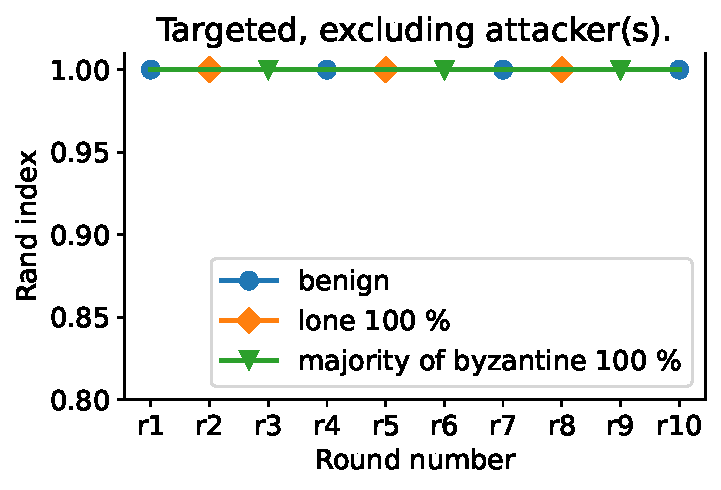
\includegraphics[width=0.47\linewidth]{figures/clustering/targeted_rand_no_attackers.pdf}
%     \quad
%     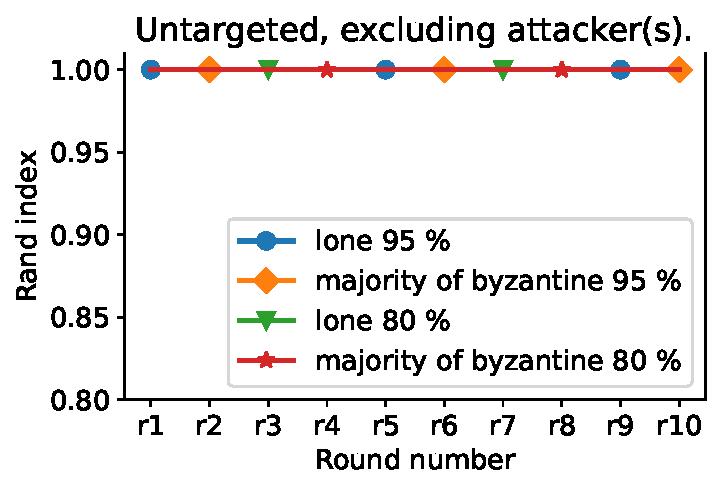
\includegraphics[width=0.47\linewidth]{figures/clustering/untargeted_rand_no_attacker.pdf}
%     \caption{
%       Clustering results compared with a partition with only benign participants.
%       The constant Rand Index of 1.0 means that all benign participants are correctly grouped according to their respective dataset, in all tested attacks.
%     }
%     \label{fig:rand_no_attackers}
%   \end{subfigure}

%   \begin{subfigure}[t]{\linewidth}
%     \centering 
%     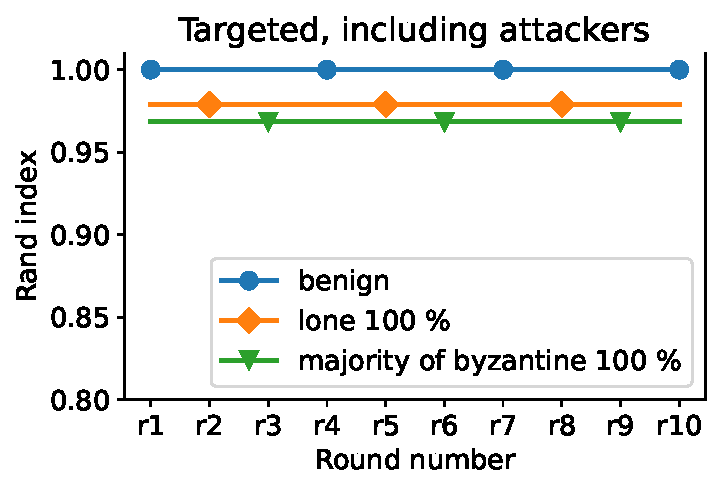
\includegraphics[width=0.47\linewidth]{figures/clustering/targeted_rand_attackers_separated.pdf}
%     \quad
%     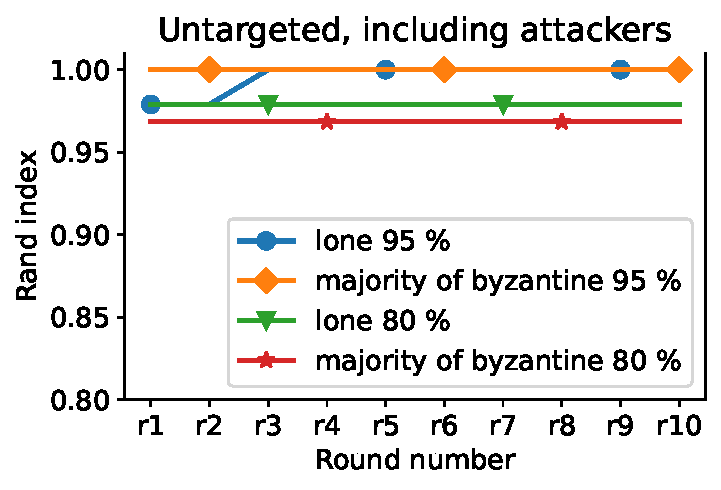
\includegraphics[width=0.47\linewidth]{figures/clustering/untargeted_rand_attackers_separated.pdf}
%     \caption{
%       Clustering results compared with a partition \textbf{with attackers grouped separately}.
%       A Rand Index of 1.0 (see untargeted attacks, \emph{noisiness} $\geq$ 95\%) means that attackers are separated from the legitimate participants, and thus cannot impact them.
%     }
%     \label{fig:rand_attackers_separated}
%   \end{subfigure}
  
%   \caption{
%     Evolution of the Rand Index over rounds, under various attack scenarios (see \Cref{sec:eval.methodo.scenarios}).
%     The Rand Index compares two partitions by quantifying how the different element pairs are grouped in each.
%     Two partitions are identical if all elements pairs are grouped or separated in the same way.
%     In this case, their Rand Index is 1.0.
%   }
%   \label{fig:rand_clustering}

% \end{figure}
% Scénarios avec des attaques. 
\subsubsection{Reputation system\label{sec:eval.results.reput}}
The reputation system weights participants inside each cluster, it aims at minimizing the weight of attackers without impacting too much the weight of benign participants. 
We first see in \Cref{fig:benign_targeted_non_expanded} that when there is no attack undergoing, all benign participants have an equal weight, underlining that the reputation system have almost no negative effect on benign participants. 
Furthermore, \Cref{fig:non_expanded_reputation}) illustrates that the reputation system is able to correctly penalize attackers, as long as they are a minority in their cluster. 
By construction, the reputation system detects the lone attacker from \Cref{fig:lone_loud_non_expanded} with a wider margin than colluding ones from \Cref{fig:byzantine_minority_loud_non_expanded}. 
Finally, the known limitation of the reputation system is apparent in \Cref{fig:byzantine_majority_loud_non_expanded}, attackers that become a majority inside a cluster gain precedence in weight and benign participants’ weight
drop. 

\begin{figure}[!t] 
  % Weights of the reputation system, before epansion.
  % Note: the images have unneeded blank space on the right.
  %       use trim+split to correct that.
  \centering
  \begin{subfigure}[t]{0.40\linewidth}
    \centering
    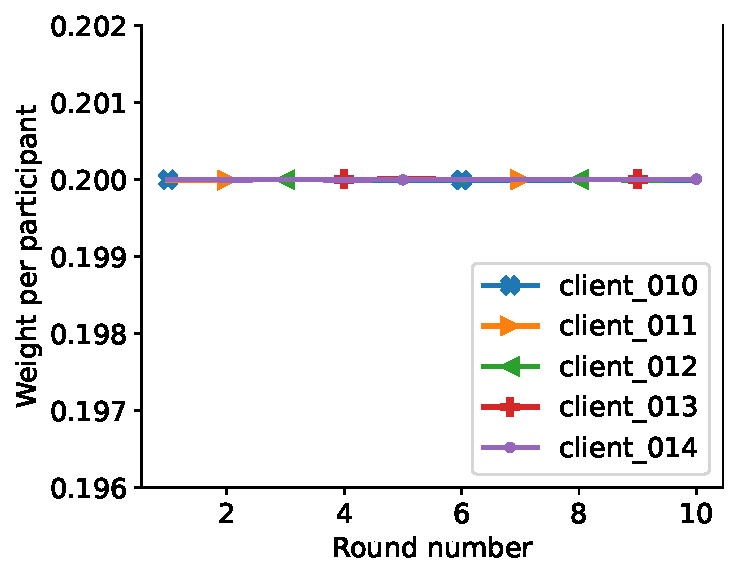
\includegraphics[trim=0 0 10pt 0,clip,width=\linewidth]{figures/reput/benign_non_expanded.pdf}
    \caption{Benign only, no difference.}
    \label{fig:benign_targeted_non_expanded}
  \end{subfigure}
  \quad 
  \begin{subfigure}[t]{0.40\linewidth}
    \centering
    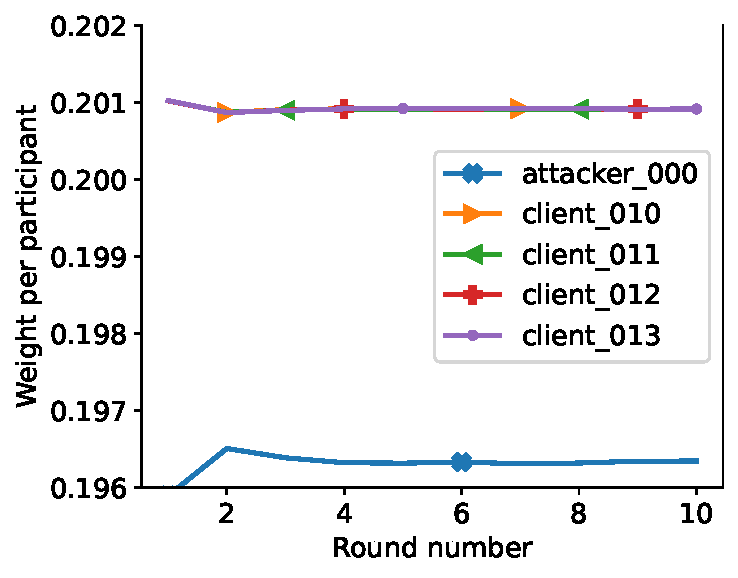
\includegraphics[trim=0 0 10pt 0,clip,width=\linewidth]{figures/reput/lone_loud_non_expanded.pdf}
    \caption{Lone attacker, clear identification.}
    \label{fig:lone_loud_non_expanded}
  \end{subfigure}

  \begin{subfigure}[t]{0.40\linewidth}
    \centering
    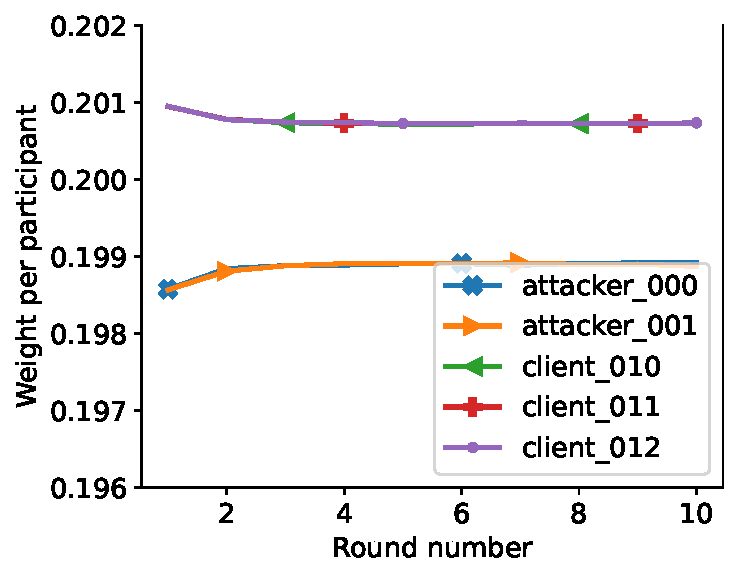
\includegraphics[trim=0 0 10pt 0,clip,width=\linewidth]{figures/reput/byzantine_minority_loud_non_expanded.pdf}
    \caption{Minority of Byzantines, less difference but still identifiable.}
    \label{fig:byzantine_minority_loud_non_expanded}
  \end{subfigure}
  \quad 
  \begin{subfigure}[t]{0.40\linewidth}
    \centering
    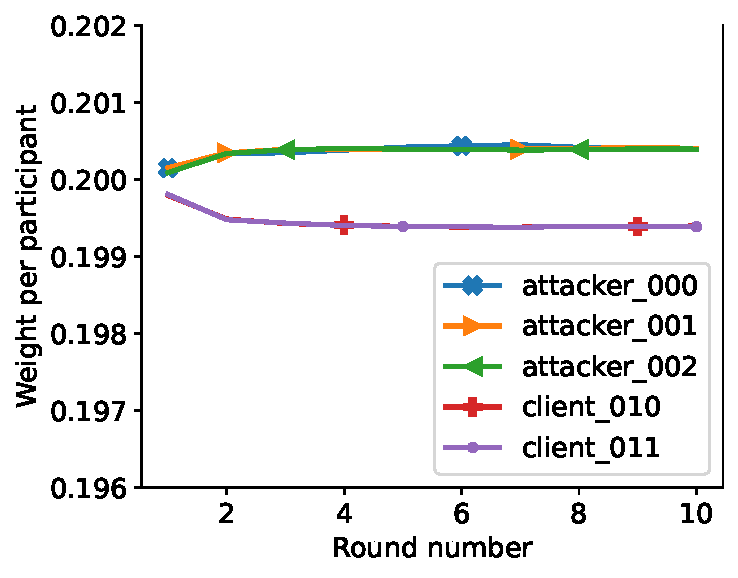
\includegraphics[trim=0 0 10pt 0,clip,width=\linewidth]{figures/reput/byzantine_majority_loud_non_expanded.pdf}
    \caption{Majority of Byzantines. Attackers gain precedence.}
    \label{fig:byzantine_majority_loud_non_expanded}
  \end{subfigure}
  \caption{
    Reputation weights $\weight$ (before expansion) given by the server for the participants of the poisoned cluster (targeted attack, 100\%) with varying number of attackers.  
    Attackers are correctly penalized when they are a minority, but gain precedence when they are the majority.}
  \label{fig:non_expanded_reputation}
\end{figure}
% Using a sigmoid function described in \Cref{sec:archi.reput}, we expand the weight differences between participants. 
One can notice the effect of the weight expansion by comparing the x-axis values between \Cref{fig:non_expanded_reputation} where weight expansion is voluntarily deactivated in the display to emphasize the difference between the different attackers' scenario, and \Cref{fig:redemption_decrease} where weight expansion is in display. 

Additionally, \Cref{fig:redemption_decrease} shows how the reputation system reacts to attackers that change their behavior over time. 
\Cref{fig:redemption_byzantine_min} feature a group of attackers going from 100\% \emph{noisiness}, to 0\%. 
They are forgiven after approximately four rounds after adapting their behavior, this rather short delay depends on the chosen $\lambda$ hyperparameter. 
On the contrary, a new attacker is detected and penalized after one round (\Cref{fig:increment_byzantine_min}), offering quick reaction to attacks. 


% \begin{figure}[!t] % REputation system weights expanded
%   \centering 

%   \begin{subfigure}[t]{.47\linewidth}
%     \centering 
%     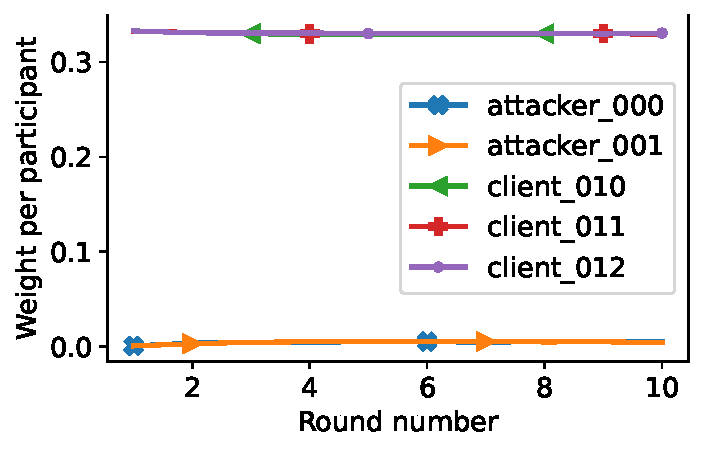
\includegraphics[trim=0 0 10pt 0,,clip,width=\linewidth]{figures/reput/byzantine_minority_loud_expanded.pdf}
%     \caption{
%       Minority of Byzantines (targeted attacks, $100\%$ \emph{noisiness}).
%       After weight expansion.
%     }
%     \label{fig:targeted_byzantine_minority_expanded_reputation}
%   \end{subfigure}
%   \quad
%   \begin{subfigure}[t]{.47\linewidth}
%     \centering 
%     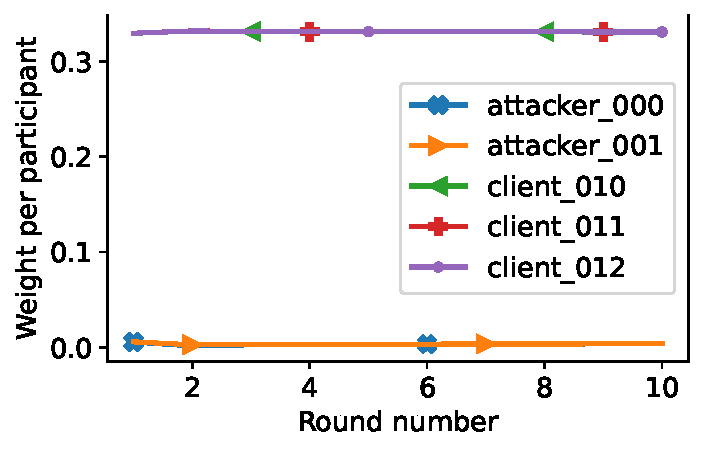
\includegraphics[trim=0 0 10pt 0,,clip,width=\linewidth]{figures/reput/untargeted_byzantine_minority_stealth_0_9.pdf}    
%     \caption{
%       Minority of Byzantines (untargeted attacks, $90\%$ \emph{noisiness}).
%       Before weight expansion.
%     }
%     \label{fig:untargeted_byzantine_minority_non_expanded_reputation}
%   \end{subfigure}

%   \caption{
%     Effect of the weight expansion function.
%     \Cref{fig:targeted_byzantine_minority_expanded_reputation} is the expanded counterpart of \Cref{fig:byzantine_minority_loud_non_expanded}, with the same scenario.
%     For \emph{loud} attacks (\Cref{fig:untargeted_byzantine_minority_non_expanded_reputation}), the difference between benign and attackers is already significant without expansion.
%   }
%   \label{fig:exploding_weights}
  
% \end{figure}

\begin{figure}[!t] % Reputation system redemption and late
  \centering 
  \begin{subfigure}[t]{.47\linewidth}
    \centering 
    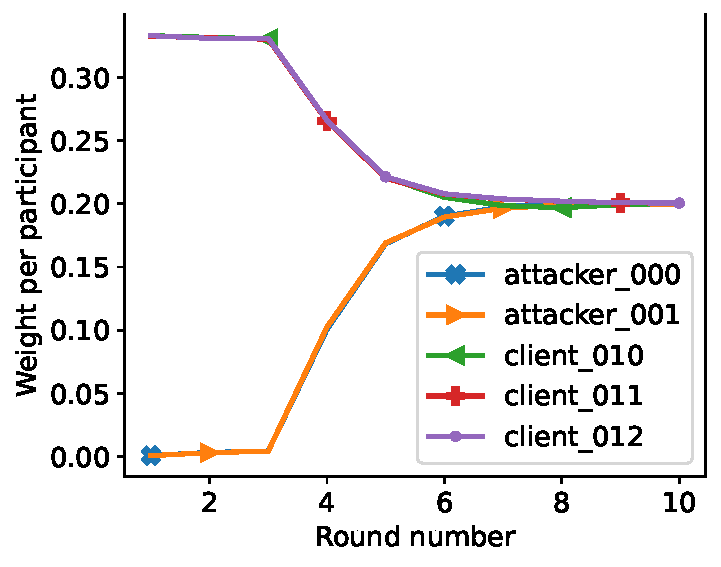
\includegraphics[trim=0 0 10pt 0,clip,width=\linewidth]{figures/reput/redemption_byzantine_min.pdf}    
    \caption{
      Attackers act with 100\% \emph{noisiness}, and become benign on round 3.
    }
    \label{fig:redemption_byzantine_min}
  \end{subfigure}
  \quad
  \begin{subfigure}[t]{.47\linewidth}
    \centering 
    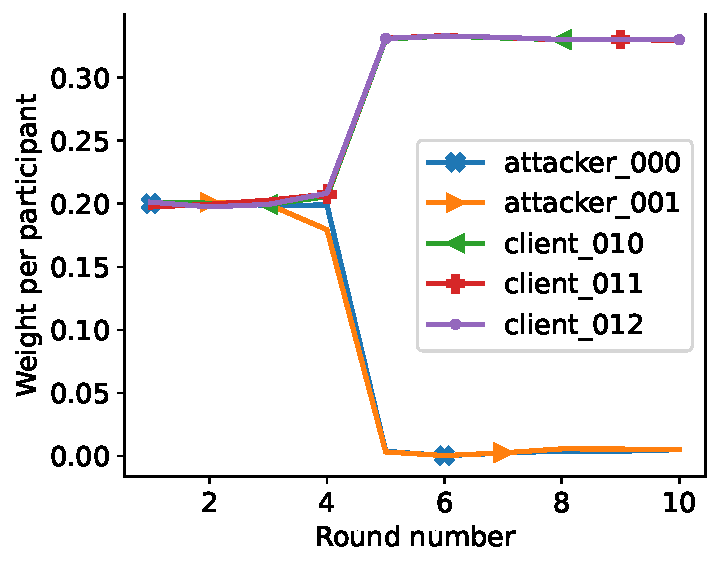
\includegraphics[trim=0 0 10pt 0,clip,width=\linewidth]{figures/reput/increment_byzantine_min.pdf}
    \caption{
      Attackers start benign, and increase \emph{noisiness} by 20\% each round when $r\geq3$.
    }
    \label{fig:increment_byzantine_min}
  \end{subfigure}
  \caption{
    Reputation weights $\weight$ (after expansion) per participant of the poisoned cluster (minority of Byzantines, targeted attack).
    Attackers are forgiven over time, and the reputation system reacts quickly to newly detected attackers.
  }
  \label{fig:redemption_decrease}

\end{figure}
%\subsubsection{Baseline comparison\label{sec:eval.results.baselines}}

\subsubsection{Comparative analysis \label{sec:eval.results.attacks}}


%\begin{table}[t]
%  % NOTE: résultats de FA_c extraits du notebook `exps/results/fedavg_per_dataset/processing.ipynb` (commit: TODO)
%      \centering
%          \caption{
%            Effects of different attack configurations (100\% \emph{noisiness}) on all baselines.
%            The attack success rate is computed over the targeted classes in targeted attacks, and over all samples otherwise (see \Cref{sec:eval.methodo.metrics}).
%            \texttt{TF} is \texttt{Trust-FIDS}, \texttt{FG} is \texttt{FoolsGold}, and \texttt{FA} is \texttt{FedAvg} (on \emph{all} participants).
%          \label{tbl:baselines_results}}
%      \bigskip
%      \setlength\tabcolsep{1ex}
%      \begin{tabular}{ll|rrr|crrrc}
%          \toprule % ---------------------------------
%          \multicolumn{2}{c|}{\multirow{2}{*}{\textbf{Attack type}}} & \multicolumn{3}{c|}{\textbf{Mean accuracy} (\%)} & \multicolumn{5}{c}{\textbf{Attack success rate} (\%)} \\
%          & & \multicolumn{1}{c}{\texttt{TF}} & \multicolumn{1}{c}{\texttt{FG}} & \multicolumn{1}{c}{\texttt{FA}}  & &\multicolumn{1}{c}{\texttt{TF}} & \multicolumn{1}{c}{\texttt{FG}} & \multicolumn{1}{c}{\texttt{FA}} & \\
%          \midrule
%          & Benign & \textbf{99.07} & 55.04 & 79.49  & & -  & - & - & \\
%          \midrule % ---------------------------------
%          % TARGETED ATTACKS
%          \multicolumn{2}{l|}{\textbf{Targeted}} & & & & & & & & \\
%            & Lone & \textbf{99.06} & 60.51 & 77.38 & & \textbf{0.00} & 93.82 & 6.73 &  \\
%            & Minority of Byzantines & \textbf{98.96} & 54.64 & 78.48 & & \textbf{0.00} & 2.97 & 9.99  &\\
%            & Majority of Byzantines & \textbf{98.28} & 85.10 & 79.40 & & 79.39 & \textbf{8.01} & 17.65 & \\
%          \midrule % ---------------------------------
%          % UNTARGETED ATTACKS
%          \multicolumn{2}{l|}{\textbf{Untargeted}} & & & & & & & &\\
%            & Lone & \textbf{98.96} & 49.56 & 78.38 & & \textbf{0.08} & 99.89 & 54.70 &\\
%            & Minority of Byzantines & \textbf{98.98} & 49.67 & 72.47 & & 0.10 & \textbf{0.04} & 44.53 &\\
%            & Majority of Byzantines & \textbf{98.96} & 69.09 & 81.87 & & \textbf{0.08} & 38.98 & 59.49 &\\          
%          \bottomrule % ---------------------------------
%      \end{tabular}
%  
%  %\end{minipage}      
%  \end{table}

\begin{table}[t]
  % NOTE: résultats de FA_c extraits du notebook `exps/results/fedavg_per_dataset/processing.ipynb` (commit: TODO)
      \centering
          \caption{
            Effects of different attack configurations (100\% \emph{noisiness}) on all baselines.
            The attack success rate is computed over the targeted classes in targeted attacks, and over all samples otherwise (see \Cref{sec:eval.methodo.metrics}).
            \texttt{TF} is \texttt{Trust-FIDS}, \texttt{FG} is \texttt{FoolsGold}, $\texttt{FA}_a$ is \texttt{FedAvg} (on \emph{all} participants), and $\texttt{FA}_c$ is \texttt{FedAvg} ideally clustered per dataset.
            The ``attack success rate'' of benign runs is provided as a baseline.
            \thecontrib's limiting scenario is marked $\ddagger$.
          \label{tbl:baselines_results}}
      \bigskip
      \setlength\tabcolsep{1ex}
      \begin{tabular}{ll|rrrr|rrrr}
          \toprule % ---------------------------------
          \multicolumn{2}{c|}{\multirow{2}{*}{\textbf{Attack type}}} & \multicolumn{4}{c|}{\textbf{Mean accuracy} (\%)} & \multicolumn{4}{c}{\textbf{Attack success rate} (\%)} \\
          & & \multicolumn{1}{c}{\texttt{TF}} & \multicolumn{1}{c}{\texttt{FG}} & \multicolumn{1}{c}{$\texttt{FA}_a$} & \multicolumn{1}{c|}{$\texttt{FA}_c$} & \multicolumn{1}{c}{\texttt{TF}} & \multicolumn{1}{c}{\texttt{FG}} & \multicolumn{1}{c}{$\texttt{FA}_a$} & \multicolumn{1}{c}{$\texttt{FA}_c$} \\
          \midrule % ---------------------------------
          % TARGETED ATTACKS
          \multicolumn{2}{l|}{\textbf{Targeted}} & & & & & & & & \\
            & Benign & \textbf{99.07} & 55.04 & 79.49 & 99.24 & \textbf{0.0}  & 5.17 & 5.10 & 0.09 \\
            & Lone & \textbf{99.06} & 60.51 & 77.38 & 99.22 & \textbf{0.00} & 93.82 & 6.73 & 0.45 \\
           & Minority of Byzantines & \textbf{98.96} & 54.64 & 78.48 & 98.33 & \textbf{0.00} & 2.97 & 9.99 & 53.40 \\
            $\ddagger$ & Majority of Byzantines & \textbf{98.28} & 85.10 & 79.40 & 98.22 & 73.39 & \textbf{8.10} & 17.65 & 59.36 \\
          \midrule % ---------------------------------
          % UNTARGETED ATTACKS
          \multicolumn{2}{l|}{\textbf{Untargeted}} & & & & & & & & \\
            & Benign & \textbf{99.07} & 55.04 & 79.49 & 99.24 & 0.09  & 0.39 & 33.30 & \textbf{0.06} \\
            & Lone & 98.96 & 49.56 & 78.38 & \textbf{99.22} &\textbf{0.08} & 99.89 & 54.70 & 0.12 \\
            & Minority of Byzantines & \textbf{98.98} & 49.67 & 72.47 & 97.69 & 0.10 & \textbf{0.04} & 44.53 & 6.26 \\
            & Majority of Byzantines & \textbf{98.96} & 69.09 & 81.87 & 75.66 & \textbf{0.08} & 38.98 & 59.49 & 94.36 \\          
          \bottomrule % ---------------------------------
      \end{tabular}
  
  %\end{minipage}      
  \end{table}

We compare \thecontrib with selected baselines under various attack scenarios in \Cref{tbl:baselines_results}. 
First, the results highlight the relevance of clustering in  \emph{practical \gls{niid}} use cases, as attacks are confined to the cluster attackers have been assigned to.
This is particularly visible in the accuracies of \thecontrib and $\texttt{FedAvg}_c$, which both maintain high accuracy overall, even for targeted attacks in majority where \thecontrib starts to falter. 
However, since \texttt{FedAvg} does not implement any mitigation strategy, its performance quickly degrades, especially by colluding attackers.

%We compare \thecontrib with selected baselines under various attack scenarios in \Cref{tbl:baselines_results}. 
%First, the results highlight the relevance of clustering in  \emph{practical \gls{niid}} use cases, as attacks are confined to the cluster attackers have been assigned to.
%This is particularly visible in the high accuracy of \thecontrib under the different attack scenarios.
%Even with a \emph{majority of Byzantines} performing targeted attacks, where \thecontrib starts to falter, the accuracy remains high since the other clusters are unaffected.
%
%Additionally, we test the attack success rate of \texttt{FedAvg} under the \emph{majority of Byzantines} scenario when all participants are trained on Bot-IoT.
%Attacks are effective at 59.37\% when targeted, and 94.37\% when untargeted, whereas \thecontrib obtains 73.39\% and 0.8\%, respectively.
%Since \texttt{FedAvg} does not implement any mitigation strategy, it is highly impacted, while not favoring attackers, in contrast to \thecontrib in the specific case of a majority of colluding targeted attackers.
%\texttt{FedAvg} with all participants, on the other hand, obtains consistently poor results, because of the absence of clustering.

The results in \Cref{tbl:baselines_results} also emphasize on \texttt{FoolsGold}'s unsuitability for \emph{practical \gls{niid}} use cases, where groups of participants sharing similar distributions can exist.
Especially in a \emph{lone attacker} scenario, any groups of similar participants are considered as colluding attackers and penalized, leading to high attack success rate, as only the attacker is considered as legitimate.
Similarly, in a \emph{minority of Byzantines} scenario, \texttt{FoolsGold} penalizes all the other clusters, leading to a model trained on Bot-IoT only.

Overall, \thecontrib shows the most consistent results, with high accuracy and low attack success rate in most scenarios, only failing against a majority of colluding participants.  
This limitation is also illustrated in \Cref{fig:trustfids_accuracy_missrate_distribution}, with a steeper drop in accuracy and miss rate when attackers outnumber benign participants in one cluster.
However, the metric distribution over the participants shows that the other clusters remain unaffected, and that the majority of benign participants continues to perform well.
This limitation is further mitigated when attackers are \emph{noisy} enough, as mentioned in the clustering analysis, since they are placed in their own cluster.
The results of \Cref{tbl:baselines_results} illustrates this, with an especially low attack success rate in \emph{untargeted} attacks, even in the \emph{majority of Byzantines} scenario. 


%In the targeted minority of Byzantine scenario, only participants from the Bot-IoT dataset are kept, while those coming from other datasets are all discarded.
%This leads to a model that is specialized on this dataset, and thus shows great results on the targeted class but an accuracy worse than \texttt{FedAvg} overall.

%Finally, in the targeted Byzantine scenario with a \emph{majority} of attackers, malicious participants are dropped and all benign are kept, leading to slightly better results than a benign \texttt{FedAvg}.
% pathological non-IID inadequate for intrusion detection (benign + attack necessary), fools gold doesn't perform well in this setting either.

%We used the following hyperparameters for the clustering: distance were measured using cosine~similarity, see \Cref{eq:cosin_sim} and the hierarchical clustering threshold is equal to 1/4th of the mean initial inter-distance. 




%\subsubsection{Resistance to attacks\label{sec:eval.results.attacks}}
% \Cref{tbl:baselines_results} presents the effect of the poisoning with varying number of attackers on the different baselines. 

% Pm : suppression des lignes dessous car exposées dans metrics et dans la légende.
% Since we mostly want to know if benign participants can be poisoned by attackers, we strip attackers from the results and only keep benign participants.  
% We then show the average accuracy of all benign participants.
% The Miss column is the average miss rate of participants as exposed in \Cref{sec:eval.methodo.metrics}.
% A complete statistic overview of these results for \thecontrib is  visually exposed in \Cref{fig:trustfids_accuracy_missrate_distribution}.
% We can see in \Cref{tbl:baselines_results} that \thecontrib successfully stops targeted attacks as long as the attackers are a minority inside their cluster: the miss rate for the lone and minority of Byzantine does not increase compared to the benign case. % deja dit, pas autant de détails
% The tipping point is when attackers outnumber legitimate participants: here, a majority of the targeted labels are misclassified. %déjà dit
% This switch can also be seen in \Cref{fig:trustfids_accuracy_missrate_distribution} with a steep degradation of the accuracy and the missrate for the participants in the targeted cluster once attackers become the majority in this cluster. 
% Also illustrated in \Cref{fig:trustfids_accuracy_missrate_distribution} however is the fact that the clients placed in the others clusters are unaffected by this event, underlining the clustering ability to limit the impact of a successful attack. 
% For untargeted attacks, we don't observe a switch when attackers become the majority. % table
% As further explained in \Cref{sec:eval.results.cluster}, untargeted attackers are noisy enough to be placed in a cluster of their own and thus have no effect on other participants. % déjà dit
% We can also see that for both untargeted and targeted attacks, the mean accuracy decreases with the number of attackers. % où ?
% Since we work with a fixed amount of data for each dataset, introducing attackers reduces the amount of data available for benign participants, which decreases their performance. % pas le cas dans nos exps...




\begin{figure}[!t]
  %\centering 
  \begin{subfigure}[t]{1.0\linewidth}
    \centering 
    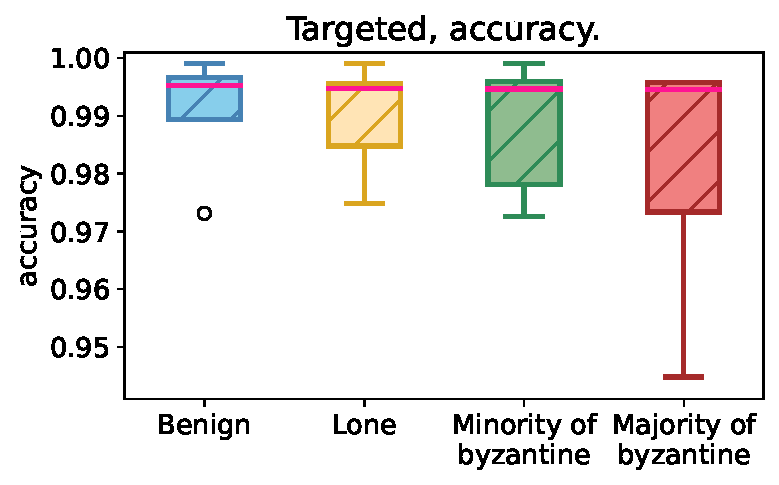
\includegraphics[width=0.47\linewidth]{figures/poisoning/trusfids_targeted_acc_all_distibutions.pdf}    
    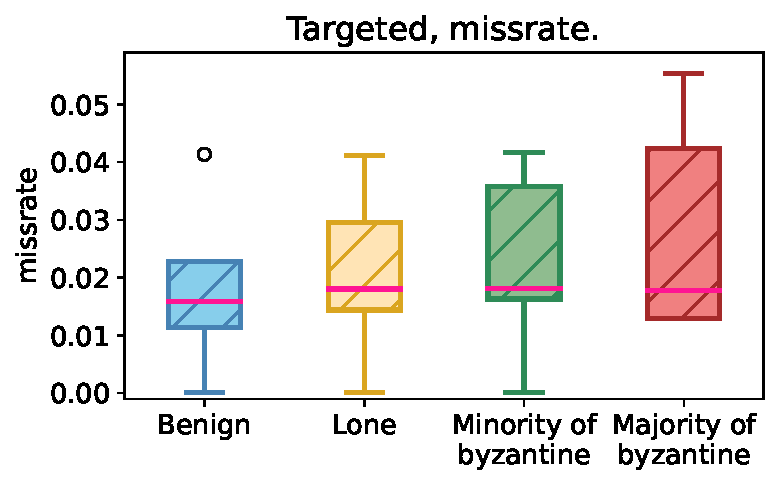
\includegraphics[width=0.47\linewidth]{figures/poisoning/trusfids_targeted_missrate_all_distibutions.pdf}   
\end{subfigure}
  \caption{
    % \thecontrib's client distribution of miss rates in different attack scenarios. 
    % The accuracy and missrate suddenly drop when attackers become the majority. 
    % Note that this effect only applies to some clients as the clients placed in others clusters are unaffected by the poisoning.
    \thecontrib's metric distribution among participants in different attack scenarios (targeted attacks, 100\% \emph{noisiness}).
    The accuracy's and miss rate's lower bounds suddenly drop when attackers outnumber benign participants in the affected cluster.
    Indeed, clients in other clusters are unaffected by the poisoning.
  }
  \label{fig:trustfids_accuracy_missrate_distribution}
  
\end{figure}